\documentclass[11pt,a4paper]{article}

% ------------------------------------------------------------------
% Packages
% ------------------------------------------------------------------
\usepackage[utf8]{inputenc}
\usepackage[T1]{fontenc}
\usepackage{lmodern}
\usepackage[margin=2.5cm]{geometry}
\usepackage{amsmath,amssymb,mathtools}
\usepackage{booktabs}
\usepackage{graphicx}
\usepackage{xcolor}
\usepackage{listings}
\usepackage{caption}
\usepackage{pgfplots}
\usepgfplotslibrary{groupplots}
\pgfplotsset{compat=1.17}
\usetikzlibrary{arrows.meta,positioning,shapes.geometric}
\usepackage[colorlinks=true,linkcolor=blue!60!black,citecolor=blue!60!black,urlcolor=blue!60!black]{hyperref}

% ------------------------------------------------------------------
% Macros
% ------------------------------------------------------------------
\newcommand{\E}{\mathbb{E}}
\newcommand{\Q}{\mathbb{Q}}
\newcommand{\ind}{\mathbf{1}}
\newcommand{\dd}{\mathrm{d}}
\newcommand{\code}[1]{\texttt{#1}}
\newcommand{\Sref}{S_{\mathrm{ref}}}

% Images extracted from the notebooks by make_figures.py ; a framed placeholder is printed while a file is missing.
\newcommand{\figfile}[2]{%
  \IfFileExists{figures/#1}{\includegraphics[width=#2]{figures/#1}}%
  {\fbox{\parbox[c][4cm][c]{#2}{\centering\small missing figure:\\ \texttt{figures/#1}}}}}

\lstset{basicstyle=\ttfamily\footnotesize, keywordstyle=\color{blue!70!black}, commentstyle=\color{gray},
        stringstyle=\color{teal}, frame=single, breaklines=true, language=Python, showstringspaces=false}

\definecolor{athena}{RGB}{31,119,180}
\definecolor{phoenix}{RGB}{214,39,40}
\definecolor{nomemory}{RGB}{255,127,14}
\definecolor{american}{RGB}{44,160,44}

% ------------------------------------------------------------------
\title{Phoenix Autocallable Notes on the CAC40 under a Calibrated Heston Model:\\
Fair Coupons, Scenarios and Greeks}
\author{Elias Benguedda}
\date{November 2026}

\begin{document}
\emergencystretch=3em
\maketitle

\begin{abstract}
We price single-underlying Phoenix autocallable notes, whose coupon is paid at each observation date where the index
is above a coupon barrier, with or without memory of the missed coupons, on the CAC40 of 12 February 2025. The
underlying follows a Heston model calibrated to the implied volatility surface (RMSE 0.42 volatility point), with a
drift read from a forward curve bootstrapped from put--call parity. The note is described by a single
parametrisation covering the observation frequency, coupon barrier and memory, autocall barrier and step-down,
non-call period, European, American continuous or American daily capital protection, airbag and capital guarantee.
The notes are priced by Monte Carlo with antithetic variates and a control variate; the American protection is
handled with the Brownian bridge crossing probability as a conditional expectation. The pricer recovers two
closed-form limit cases and an exact identity with the snowball Athena. We report the fair coupon (price at par) of
19 variants together with their scenario statistics: the base Phoenix (4 years, quarterly observations, memory,
coupon barrier at 70\%, autocall at 100\%, European protection at 60\%) pays 6.04\% a year, is called after one
quarter with probability 55.4\% and loses capital with probability 5.2\%. The memory is worth 0.37 point of coupon
and an American protection costs 1.14 points. The note is almost Delta-neutral at the money, short volatility
($-0.33$ per vol point on a nominal of 100) and short dividends ($-0.32$ per point of carry).
\end{abstract}

\clearpage
\tableofcontents
\newpage

% ==================================================================
\section{Introduction}
% ==================================================================
In an AutoCallable note, the investor
receives coupons well above the risk-free rate, and the note is redeemed early (``called'') as soon as the index is
above a reference level on an observation date. The coupon is financed by selling a down-and-in put. If the note
is never called and the index ends below a protection barrier, the investor bears the loss of the index.

This report studies the \textbf{Phoenix}, whose coupon is paid at each observation date where the index is above a
coupon barrier, lower than the autocall barrier, usually with a \emph{memory} of the missed coupons. The other main
family, the Athena, whose coupon is paid only when the note is called, is treated in a companion report
\cite{benguedda2026athena}.
On top of this structure, issuers combine many features: observation frequency, step-down of the autocall barrier,
non-call period, European or American protection, airbag, capital guarantee. We will have a look on how to price
these different versions in a single framework, on real market data, and measure how each feature moves the fair
coupon, the probabilities of the scenarios and the Greeks.

The model is the Heston model calibrated in \cite{benguedda2026heston} to the CAC40 implied volatility surface, and the Monte Carlo engine is the one used for barrier options in \cite{benguedda2026barrier}. The scripts and
notebooks are open source; Section~\ref{sec:implementation} describes the code.

% ==================================================================
\section{Products}\label{sec:products}
% ==================================================================

\subsection{Common structure}
A note of nominal $N$ on an index $S$ has an initial fixing $\Sref$ and observation dates
$0 < t_1 < \dots < t_n = T$. The performance at $t_k$ is $P_k = S_{t_k}/\Sref$. All barriers are fractions of
$\Sref$: autocall barriers $B^{\mathrm{call}}_k$, coupon barriers $B^{\mathrm{cpn}}_k$ and protection
barrier $B^{\mathrm{prot}}$. The dates $t_k$ with $t_k \ge t_{\mathrm{nc}}$ are callable, $t_{\mathrm{nc}}$ being the
end of the non-call period; the maturity is always callable. The first callable date where
$P_k \ge B^{\mathrm{call}}_k$ is the call date $\tau$.

\paragraph{Redemption at maturity.} If the note is never called, it is redeemed at $T$ at
\begin{equation}\label{eq:redemption}
R_T = N\left[(1 - \ind_{\mathrm{KI}}) + \ind_{\mathrm{KI}}\,\max\!\Big(\phi,\ \min\big(1,\ P_T/K_{\mathrm{put}}\big)\Big)\right],
\end{equation}
where $\ind_{\mathrm{KI}}$ is the knock-in event of the protection, $K_{\mathrm{put}}$ the strike of the short put
and $\phi$ the capital floor. The knock-in event is
\begin{itemize}
\item \emph{European protection}: $P_T < B^{\mathrm{prot}}$;
\item \emph{American protection}: the index touches $B^{\mathrm{prot}}\Sref$ at any time before maturity,
continuously or on daily closes.
\end{itemize}
The standard note has $K_{\mathrm{put}} = 1$ and $\phi = 0$: below the barrier, the investor receives
$N P_T$ and the redemption jumps from $N$ to $N B^{\mathrm{prot}}$ at the barrier. The \emph{airbag} note has
$K_{\mathrm{put}} = B^{\mathrm{prot}}$: the redemption is continuous at the barrier and equal to
$N P_T / B^{\mathrm{prot}}$ below it. A \emph{capital guarantee} sets $\phi > 0$. Figure~\ref{fig:redemption}
draws the three profiles.

\begin{figure}[h]
\centering
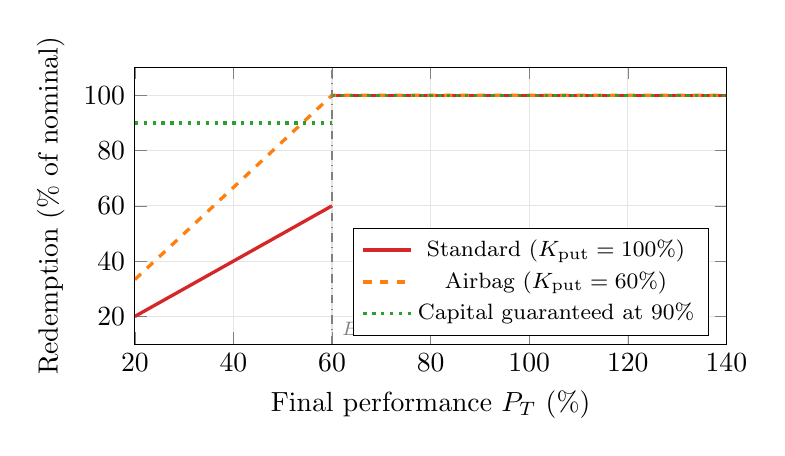
\begin{tikzpicture}
\begin{axis}[width=0.75\textwidth, height=0.42\textwidth, xmin=20, xmax=140, ymin=10, ymax=110,
             xlabel={Final performance $P_T$ (\%)}, ylabel={Redemption (\% of nominal)},
             grid=major, grid style={gray!20}, legend pos=south east, legend style={font=\footnotesize}]
\addplot[phoenix, very thick] coordinates {(20,20) (60,60)};
\addplot[phoenix, very thick, forget plot] coordinates {(60,100) (140,100)};
\addplot[nomemory, very thick, dashed] coordinates {(20,33.33) (60,100) (140,100)};
\addplot[american, very thick, dotted] coordinates {(20,90) (60,90)};
\addplot[american, very thick, dotted, forget plot] coordinates {(60,100) (140,100)};
\draw[gray, dashdotted] (axis cs:60,10) -- (axis cs:60,110) node[pos=0.06, right, font=\scriptsize] {$B^{\mathrm{prot}} = 60\%$};
\legend{Standard ($K_{\mathrm{put}} = 100\%$), Airbag ($K_{\mathrm{put}} = 60\%$), Capital guaranteed at 90\%}
\end{axis}
\end{tikzpicture}
\caption{Redemption at maturity of a note that was never called, European protection at 60\% (the last coupon is
paid on top of it if $P_T \ge B^{\mathrm{cpn}}_n$).}
\label{fig:redemption}
\end{figure}

\subsection{Phoenix}
The Phoenix pays at each observation date $t_k \le \tau$ (and $t_k \le T$) the coupon
\begin{equation}
N\, c\,(t_k - t_{k-1})\, \ind_{\{P_k \ge B^{\mathrm{cpn}}_k\}}
\end{equation}
and, with memory, the coupons of all the previous dates since the last payment. When the note is called, it is
redeemed at $N$. With $B^{\mathrm{cpn}}_k = 0$, the coupon is unconditional; with
$B^{\mathrm{cpn}}_k = B^{\mathrm{call}}_k$ and memory, a coupon is paid only at the call date and its amount is
$c\, t_k$: the Phoenix is then exactly a snowball Athena (Table~\ref{tab:validation} checks it numerically).

\subsection{Parametrisation}
Table~\ref{tab:parameters} lists the parameters of the class \code{Phoenix}; every variant of
Section~\ref{sec:phoenix} is one of these parameters changed.

\begin{table}[h]
\centering
\resizebox{\textwidth}{!}{%
\begin{tabular}{@{}lll@{}}
\toprule
\textbf{Feature} & \textbf{Parameter} & \textbf{Values} \\
\midrule
Maturity, initial fixing, nominal & \code{maturity}, \code{initial\_fixing}, \code{nominal} & years, index level, 100 \\
Observation dates & \code{frequency} or \code{observation\_dates} & monthly to annual, or any list ending at $T$ \\
Coupon rate & \code{coupon\_rate} & per annum, fraction of the nominal \\
Coupon condition & \code{coupon\_barrier}, \code{memory} & fraction of $\Sref$ (scalar or one per date), True / False \\
Autocall barrier & \code{autocall\_barrier}, \code{step\_down} & fraction of $\Sref$, decrease per observation \\
Non-call period & \code{first\_call\_date} & years \\
Capital protection & \code{protection\_barrier}, \code{protection\_type} & fraction of $\Sref$; \code{european}, \code{american}, \code{american\_discrete} \\
Airbag, guarantee & \code{put\_strike}, \code{floor} & fraction of $\Sref$, fraction of the nominal \\
\bottomrule
\end{tabular}}
\caption{Parameters of the Phoenix (\code{Products/Phoenix/phoenix.py}).}
\label{tab:parameters}
\end{table}

\clearpage
% ==================================================================
\section{Market Data and Model}\label{sec:model}
% ==================================================================
The data are the CAC40 option chain of 12 February 2025 (spot $S_0 = 8042.19$, 142 quotes on 13 expiries from
9 days to 4.86 years) and the EURIBOR 6M zero-coupon curve. The forward curve $F(0,t)$ is bootstrapped from
put--call parity with a piecewise constant borrow-plus-dividend yield $q(t)$ \cite{benguedda2026heston}; its
integral reaches 0.136 at 4.86 years, so dividends lower the 4-year forward by about 11\% with respect to a zero
carry. Under $\Q$,
\begin{equation}
\frac{\dd S_t}{S_t} = \partial_t \ln F(0,t)\,\dd t + \sqrt{v_t}\,\dd W^S_t, \qquad
\dd v_t = \kappa(\theta - v_t)\,\dd t + \xi \sqrt{v_t}\,\dd W^v_t, \qquad \dd\langle W^S, W^v\rangle_t = \rho\,\dd t,
\end{equation}
with the parameters of Table~\ref{tab:heston}. The notes are struck at the money: $\Sref = S_0 = 8042.19$, and
$\Sref$ stays fixed when the Greeks bump the market. All the dates of the 4-year notes lie before the last listed
expiry (4.86 years).

\begin{table}[h]
\centering
\begin{tabular}{@{}cccccc@{}}
\toprule
$v_0$ & $\theta$ & $\kappa$ & $\xi$ & $\rho$ & IV RMSE \\
\midrule
0.0197 & 0.0438 & 1.308 & 0.482 & $-0.605$ & 0.421 vol pts \\
\bottomrule
\end{tabular}
\caption{Heston parameters calibrated on the CAC40 surface of 12 February 2025 \cite{benguedda2026heston}.}
\label{tab:heston}
\end{table}


\clearpage
% ==================================================================
\section{Pricing Method}\label{sec:method}
% ==================================================================

\subsection{Simulation}
The paths of $(S, v)$ are simulated with an Euler full truncation scheme on a weekly grid (52 steps a year,
208 steps for 4 years), the drift over each step being $\ln(F(0,t_{i+1})/F(0,t_i))$, so that
$\E[S_t] = F(0,t)$ at every date. $N = 50{,}000$ paths with antithetic variates are used (seed 42); prices and
standard errors are computed on the 25{,}000 independent pair averages. The observation dates are rounded to the
grid; with weekly steps, every monthly, quarterly, semi-annual and annual date falls within half a week of its
contractual date.

\subsection{Cash flows and protection}
For each path, the note is followed through its observation dates: at each date, the coupon is paid if the
performance is above the coupon barrier (with the unpaid coupons if the note has a memory), then the note is called
if the performance is above the autocall barrier. Each cash flow is discounted with $D(0,t_k) = e^{-r(t_k) t_k}$.
The knock-in indicator of \eqref{eq:redemption} is
\begin{itemize}
\item \emph{European}: $\ind_{\{P_T < B^{\mathrm{prot}}\}}$;
\item \emph{American continuous}: replaced by its conditional probability given the simulated path,
$1 - \prod_i (1 - p_i)$, where
$p_i = \exp\!\big(-2 \ln(S_{t_i}/H) \ln(S_{t_{i+1}}/H) / (v_{t_i}\Delta t)\big)$ is the probability that the
Brownian bridge of $\ln S$ touches $H = B^{\mathrm{prot}}\Sref$ between two grid dates \cite{beaglehole1997};
\item \emph{American daily}: the barrier is checked on a daily grid (252 steps a year).
\end{itemize}

\subsection{Variance reduction}
Besides antithetic variates, the discounted European put struck at $B^{\mathrm{prot}}\Sref$, whose Heston price
is known semi-analytically (Lewis formula), is used as a control variate with an optimal coefficient estimated on
the paths.

\subsection{Fair coupon and scenario statistics}
On a fixed set of paths, the call dates do not depend on the coupon, and every cash flow is affine in the coupon
rate $c$: the price is $V(c) = V(0) + c\,(V(1) - V(0))$, and the coupon that prices the note at par is
\begin{equation}
c^\star = \frac{N - V(0)}{V(1) - V(0)},
\end{equation}
obtained with two valuations. It excludes the issuer margin and funding spread. The same paths give the
probability of a call at each date, the probability to reach maturity, the probability of a capital loss
($\ind_{\mathrm{KI}} = 1$ and $P_T < K_{\mathrm{put}}$), the expected loss at maturity, the expected life
$\E[\min(\tau, T)]$ and the expected number of coupons.

\subsection{Greeks}
The Greeks are central finite differences with common random numbers \cite{glasserman2004}, on a nominal of 100:
Delta and Gamma (spot $\pm 1\%$, carry kept), Vega and Volga ($\sqrt{v_0}$ and $\sqrt{\theta}$ shifted by
$\pm 1$ vol point), Vanna, Rho ($\pm 10$bp on the zero curve, per $+1\%$), Dividend ($\pm 10$bp on $q(t)$, per
$+1\%$) and Theta (dates moved by one day). Delta is given per index point: multiply by $S_0/100 = 80.4$ for the
value change of a 1\% move. Each Greek is reported with its Monte Carlo standard error.

\subsection{Validation}
Two limit cases have a closed form and one an exact counterpart (Table~\ref{tab:validation}). In a flat
Black--Scholes market ($S_0 = \Sref = 100$, $r = 3\%$, $q = 1\%$, $\sigma = 20\%$, $T = 2$, $N = 100$, Heston with
$v_0 = \theta = \sigma^2$ and $\xi = 10^{-4}$, $10^5$ paths):
\begin{itemize}
\item a Phoenix never called (autocall barrier out of reach) with unconditional quarterly coupons and a European
protection at $B = 60$ is worth the sum of its discounted coupons plus
$N D(T) - \frac{N}{\Sref}\left[\mathrm{Put}(B) + (\Sref - B)\,\mathrm{DigitalPut}(B)\right]$;
\item a Phoenix called for sure at $t_1$ is worth $N(1 + c\,t_1) D(t_1)$.
\end{itemize}
On the CAC40, the Phoenix with memory and $B^{\mathrm{cpn}} = B^{\mathrm{call}}$ must have exactly the price of the
snowball Athena with the same dates.

\begin{table}[h]
\centering
\resizebox{\textwidth}{!}{%
\begin{tabular}{@{}lrrrr@{}}
\toprule
\textbf{Case} & \textbf{Reference} & \textbf{Monte Carlo} & \textbf{Std error} & \textbf{Error / std error} \\
\midrule
Phoenix never called, unconditional 6\% coupon (flat) & 104.2404 & 104.2515 & 0.0141 & 0.79 \\
Phoenix called for sure at $t_1 = 0.25$, $c = 6\%$ (flat) & 100.742 & 100.742 & 0 & exact \\
Phoenix with memory, $B^{\mathrm{cpn}} = B^{\mathrm{call}}$ vs snowball Athena (CAC40) & 98.7669 & 98.7669 & 0.0585 & identical paths \\
\bottomrule
\end{tabular}}
\caption{Validation of the pricer.}
\label{tab:validation}
\end{table}


\clearpage
% ==================================================================
\section{Phoenix : Base case}\label{sec:phoenix}
% ==================================================================


Let us consider, under the risk-neutral measure $\mathbb{Q}$, the general
case of a Phoenix in the base case, on a nominal of 1, with $N$ observation
dates, a coupon $c$ per period, a coupon barrier $B_c$, an autocall barrier
$B_{ac}$ and a protection barrier $B_p$, with $B_p \le B_c \le B_{ac}$. As
for the Athena, we denote by
\begin{equation}
  E_i = \bigcap_{j=1}^{i-1} \{X_j < B_{ac}\}, \qquad i = 1, \dots, N,
  \qquad E_1 = \Omega,
\end{equation}
the event that the product has not been called before date $t_i$. The
event $\{\tau = t_i\}$ of an early redemption at date $t_i < T$ is then
$E_i \cap \{X_i \geq B_{ac}\}$, and $\{\tau = T\} = E_N$. With memory, the
coupon paid at $t_i$ covers all the periods since the last payment: it is
$c\, m_i$, with
\begin{equation}
  m_i = i - \max\bigl(\{0\} \cup \{ j < i : X_j \ge B_c \}\bigr),
\end{equation}
and $m_i = 1$ without memory.

\subsection{Price of the Phoenix}

For a coupon $c$, the price of the Phoenix at inception is the sum of its
discounted coupons and of its discounted redemption,
\begin{equation}
  P_0 = \mathbb{E}^{\mathbb{Q}}\Bigl[ \sum_{t_i \le \tau} D(t_i)\, c\, m_i\,
        \ind_{\{X_i \ge B_c\}} + D(\tau)\, \Pi_\tau \Bigr],
\end{equation}
which, writing the autocall events explicitly, expands as
\begin{align}
  P_0 = {}& \sum_{i=1}^{N} D(t_i)\, c\,
          \mathbb{E}^{\mathbb{Q}}\bigl[ m_i\, \ind_{E_i \cap \{X_i \geq B_c\}} \bigr] \nonumber \\
        & + \sum_{i=1}^{N-1} D(t_i)\,
          \mathbb{Q}\bigl( E_i \cap \{X_i \geq B_{ac}\} \bigr) \nonumber \\
        & + D(T)\,
          \mathbb{Q}\bigl( E_N \cap \{X_N \geq B_p\} \bigr) \nonumber \\
        & + D(T)\,
          \mathbb{E}^{\mathbb{Q}}\bigl[ X_N \, \ind_{E_N \cap \{X_N < B_p\}} \bigr].
  \label{eq:phoenix-price-explicit}
\end{align}
The first term is the strip of conditional coupons, the second corresponds
to an early redemption at date $t_i$, the third to the repayment of the
notional at maturity, and the last one to the capital loss scenario.
Contrary to the Athena, the coupon is not attached to the redemption: it is
paid as long as the note is alive and the index above $B_c$, including in
scenarios that end with a capital loss.

\subsection{Linearity in the coupon and embedded put}

The price of the Phoenix is also affine in the coupon: the coupon affects
the amounts paid, never the redemption time $\tau$ nor the dates where a
coupon is paid, which depend on the path of the underlying alone. On the
event $E_N$, the terminal payoff can be rewritten, since $B_p < 1$, as
\begin{equation}
  \Pi_T = 1 + c\, m_N\, \ind_{\{X_N \geq B_c\}}
        - (1 - X_N)^+ \, \ind_{\{X_N < B_p\}} ,
  \label{eq:phoenix-terminal-payoff}
\end{equation}
where the last term is again the down-and-in put with strike $100\%$ and
barrier $B_p$ observed at maturity, sold by the investor. Substituting
\eqref{eq:phoenix-terminal-payoff} into \eqref{eq:phoenix-price-explicit}
yields the decomposition
\begin{equation}
  P_0 = \underbrace{\mathbb{E}^{\mathbb{Q}}\bigl[ D(\tau) \bigr]}_{\text{notional}}
      + c \underbrace{\sum_{i=1}^{N} D(t_i)\,
        \mathbb{E}^{\mathbb{Q}}\bigl[ m_i\, \ind_{E_i \cap \{X_i \geq B_c\}} \bigr]}_{B \ (\text{coupons})}
      - \underbrace{D(T)\, \mathbb{E}^{\mathbb{Q}}\Bigl[ (1 - X_N)^+ \,
        \ind_{\{X_N < B_p\}}\, \ind_{E_N} \Bigr]}_{\mathrm{PDI}^{ac}} ,
  \label{eq:phoenix-pdi}
\end{equation}
that is
\begin{equation}
  P_0 = A + c\, B,
  \qquad
  A = \mathbb{E}^{\mathbb{Q}}\bigl[ D(\tau) \bigr] - \mathrm{PDI}^{ac}.
\end{equation}
The zero-coupon part $A$ does not depend on the coupon condition: for the
same dates and the same autocall and protection barriers, \emph{the Phoenix
and the Athena have the same $A$}. They only differ through the value $B$
of a unit coupon. Two limit cases bound it:
\begin{itemize}
  \item with $B_c = 0$ (unconditional coupon), $m_i = 1$ and
        $B = \sum_i D(t_i)\, \mathbb{Q}(E_i)$, a strip of coupons knocked
        out at the call;
  \item with $B_c = B_{ac}$ and memory, $X_j < B_c$ for every $j < i$ on
        $E_i$, so that $m_i = i$ and $B$ is exactly the $B$ of the snowball
        Athena.
\end{itemize}

\subsection{Fair coupon}

As for the Athena, the fair coupon for a target price $P^\star$ ($1$, or
$1 - m$ with an issuer margin $m$) is
\begin{equation}
  \boxed{\,c^\star = \frac{P^\star - A}{B}
  = \frac{P^\star - \mathbb{E}^{\mathbb{Q}}\bigl[ D(\tau) \bigr] + \mathrm{PDI}^{ac}}{B}\,}
  \label{eq:fair-coupon}
\end{equation}
and a single Monte Carlo simulation provides $A$ and $B$. Since $A$ is
shared with the Athena of the same dates, the ratio of the two fair coupons
is the inverse ratio of the coupon values,
\begin{equation}
  \frac{c^\star_{\mathrm{Phoenix}}}{c^\star_{\mathrm{Athena}}}
  = \frac{B_{\mathrm{Athena}}}{B_{\mathrm{Phoenix}}} .
\end{equation}
On the base case, the quarterly snowball Athena pays 10.54\% and the Phoenix
6.04\%: a unit coupon is worth 1.75 times more in the Phoenix, because it is
also paid in the scenarios where the index stays between $B_c$ and $B_{ac}$.

\subsection{Remarks on the embedded put and on the coupons}

The put $\mathrm{PDI}^{ac}$ is the same as in the Athena: knocked out by
the autocall, bounded by the European down-and-in put, which decomposes
into a vanilla put struck at the barrier and a digital put,
\begin{equation}
  (1 - X_N)^+ \, \ind_{\{X_N < B_p\}}
  = (B_p - X_N)^+ + (1 - B_p)\, \ind_{\{X_N < B_p\}}.
\end{equation}
The coupons add a second exposure to the shape of the distribution: each
coupon is a digital call struck at $B_c$, knocked out by an earlier call.
Without memory, $B = \sum_i D(t_i)\, \mathbb{Q}(E_i \cap \{X_i \ge B_c\})$;
the memory can only increase it, up to $\sum_i i\, D(t_i)\,
\mathbb{Q}(E_i \cap \{X_i \ge B_c\})$. Both strips are sensitive to the skew
around $B_c$.



\subsection{Structuration :}

From the investor's perspective, the basic Phoenix note is composed of:
\begin{itemize}
  \item a long position in an \emph{autocallable zero-coupon note} with
        maximal maturity $T$, which repays the notional at the first
        observation date $t_i$ such that $X_i \geq B_{ac}$, and at maturity
        otherwise;
  \item a long position in a \emph{strip of digital coupons} paying $c$ (or
        $c\, m_i$ with memory) at each date $t_i$ where $X_i \ge B_c$, knocked
        out when the product is autocalled;
  \item a short position in a \emph{down-and-in put} (PDI) with strike
        $100\%$ and barrier $B_p$ observed at maturity, which is knocked
        out whenever the product is autocalled.
\end{itemize}


\subsection{Sensitivity analysis :}

We will now look at the different sensitivities of the product and what are the impacts of a move on certain
parameters on $c$. We are now thinking from the investor point of view and with an already contracted note.


\subsection*{Volatility}

The investor is short the PDI, whose price increases with volatility: he is short vega. The digital coupons, struck
at $B_c = 70\%$ below the spot, also lose value when the volatility rises, since the index is less likely to stay
above the coupon barrier. The base note loses 0.33 per vol point.

If the product is not contracted yet, a higher volatility makes the put more expensive, and the fair coupon $c$
increases.


\subsection*{Protection barrier}

If the protection barrier is higher, then it is more probable to cross it and it reduces the price of the note. The
effect on the coupon $c$ is that it is increased: 5.16\% at 50\%, 6.04\% at 60\%, 6.85\% at 70\%.


\subsection*{Recall Barrier}

If the recall barrier is increased, it is less probable to be recalled before maturity: the investor keeps the put
longer, and the fair coupon $c$ increases (5.46\% with an autocall barrier at 90\%, 6.04\% at 100\%). Contrary to
the Athena, a longer life also means more coupons, which limits the effect; a step-down of the autocall barrier,
which shortens the coupon stream, raises the fair coupon (6.20\%).


\subsection*{Coupon barrier}

If the coupon barrier is increased, fewer coupons are paid and the fair coupon $c$ increases: 5.43\% at 50\%, 6.04\%
at 70\%, 6.67\% at 80\%, and 5.13\% for an unconditional coupon.


\subsection*{Memory}

The memory pays back the missed coupons as soon as the index comes back above $B_c$: it is worth 0.37 point of coupon
at a coupon barrier of 70\% (6.04\% instead of 6.41\% without memory), and 2.41 points at 90\%.


\subsection*{Dividend}

If the underlying asset increases its dividend, the forward decreases: the put is more valuable, the coupons and the
calls less likely, and the fair coupon $c$ increases. The investor does not receive the dividends. The exposure is a
third of the Athena one ($-0.32$ per point of carry against $-1.12$), the coupons being paid on a shorter horizon.


\subsection*{Spread}




\subsection*{Risk free rate}




\subsection*{Maturity}




\subsection*{Skew}






\subsection*{Correlation}





\subsection{Pricing : A numerical example}


Let us now consider a synthetic Phoenix issued by a risky issuer, which
requires taking into account the credit spread of the issuer. The product
is written on the CAC~40 index (dividends not reinvested). Its initial level
is fixed on 31 January 2025 and it matures in November 2027. The underlying
is observed quarterly: at each observation date, a coupon $c$ is paid if the
index closes at or above the coupon barrier $B_c = 70\%$ of its initial
level, together with the coupons missed since the last payment (memory),
and the product is redeemed early if the index closes at or above $100\%$
of its initial level. If the product has not been called, the investor
receives at maturity the last coupon if the index is at or above the coupon
barrier, the notional if it is at or above the protection barrier
$B_p = 60\%$, and the notional reduced by the full decline of the index
otherwise.

\subsubsection{Model}

\subsubsection{Pricing}

\subsubsection{Sensitivities}

\subsection{Features of Phoenix products}

\subsubsection{Exercise frequency}

\subsubsection{Memory}

\subsubsection{Step-down barrier}

\subsubsection{Airbag}

\subsubsection{Buffer}

\subsubsection{Guaranteed capital}

\subsubsection{Coupon range accrual}

\subsubsection{Duo mechanism}

\subsubsection{Look back}



\begin{figure}[h]
\centering
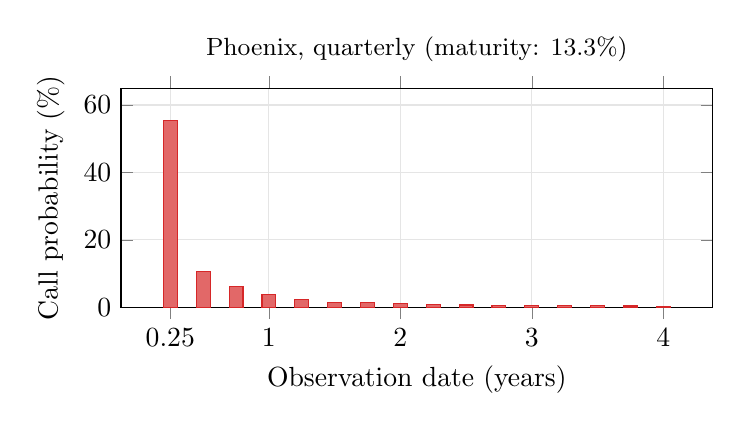
\begin{tikzpicture}
\begin{axis}[width=0.75\textwidth, height=0.36\textwidth, ymin=0, ymax=65, ylabel={Call probability (\%)},
  grid=major, grid style={gray!20}, title style={font=\small}, ybar, bar width=5pt,
  xlabel={Observation date (years)}, xtick={0.25,1,2,3,4}, title={Phoenix, quarterly (maturity: 13.3\%)}]
\addplot[fill=phoenix!70, draw=phoenix] coordinates {(0.25,55.43) (0.5,10.63) (0.75,6.24) (1,3.86) (1.25,2.21) (1.5,1.57)
  (1.75,1.41) (2,1.13) (2.25,0.82) (2.5,0.69) (2.75,0.59) (3,0.51) (3.25,0.46) (3.5,0.47) (3.75,0.39) (4,0.30)};
\end{axis}
\end{tikzpicture}
\caption{Base Phoenix: probability of being called at each observation date (autocall barrier at 100\%).}
\label{fig:call_probabilities}
\end{figure}

The base Phoenix has a maturity of 4 years, quarterly observations, a coupon of 6\% a year (1.5\% a quarter)
with memory and a coupon barrier at 70\%, an autocall barrier at 100\% and a European protection at 60\%. Its price
is $99.963 \pm 0.099$ (95\%) and its fair coupon $6.04\%$ a year. 55.4\% of the notes are called after one
quarter (Figure~\ref{fig:call_probabilities}), the expected life is 1.03 years, 3.28 coupons are paid on
average, 13.3\% of the notes reach maturity and 5.2\% lose capital, with an expected loss of 3.05\%.

\begin{figure}[h]
\centering
\figfile{phoenix_scenarios.png}{0.9\textwidth}
\caption{Base Phoenix: simulated paths of the performance, grouped by outcome.}
\label{fig:phoenix_scenarios}
\end{figure}

\subsection{All the forms of the Phoenix}
Table~\ref{tab:phoenix_variants} changes one feature of the base case at a time. All prices are computed at the same
coupon of 6\%; the fair coupon is the comparable quantity.

\begin{table}[h]
\centering
\resizebox{\textwidth}{!}{%
\begin{tabular}{@{}lrrrrrrr@{}}
\toprule
\textbf{Variant} & \textbf{Price at 6\%} & \textbf{Fair coupon} & \textbf{P(maturity)} & \textbf{P(loss)} & \textbf{E[loss]} & \textbf{E[life]} & \textbf{E[coupons]} \\
 & & \textbf{(\% p.a.)} & \textbf{(\%)} & \textbf{(\%)} & \textbf{(\%)} & \textbf{(y)} & \\
\midrule
Base (quarterly, memory, CB 70\%) & 99.96 & 6.04 & 13.29 & 5.22 & 3.05 & 1.03 & 3.28 \\
No memory & 99.67 & 6.41 & 13.29 & 5.22 & 3.05 & 1.03 & 3.28 \\
Coupon barrier 50\% & 100.54 & 5.43 & 13.29 & 5.22 & 3.05 & 1.03 & 3.83 \\
Coupon barrier 60\% & 100.30 & 5.67 & 13.29 & 5.22 & 3.05 & 1.03 & 3.61 \\
Coupon barrier 80\% & 99.49 & 6.67 & 13.29 & 5.22 & 3.05 & 1.03 & 2.80 \\
Coupon barrier = autocall barrier (= snowball Athena) & 97.80 & 10.54 & 13.29 & 5.22 & 3.05 & 1.03 & 0.87 \\
Unconditional coupon (CB 0\%) & 100.87 & 5.13 & 13.29 & 5.22 & 3.05 & 1.03 & 4.13 \\
Monthly observations & 99.91 & 6.19 & 7.77 & 3.13 & 1.83 & 0.59 & 5.53 \\
Semi-annual observations & 100.22 & 5.82 & 18.61 & 6.97 & 4.08 & 1.48 & 2.38 \\
Annual observations & 100.62 & 5.63 & 25.70 & 9.06 & 5.27 & 2.06 & 1.67 \\
Autocall barrier 90\% & 100.19 & 5.46 & 3.13 & 1.70 & 1.01 & 0.42 & 1.37 \\
Step-down 1.25\% per quarter & 99.86 & 6.20 & 7.14 & 4.29 & 2.54 & 0.84 & 2.62 \\
Non-call 1 year & 100.86 & 5.46 & 22.06 & 8.42 & 4.92 & 1.89 & 6.21 \\
Protection 50\% & 100.71 & 5.16 & 13.29 & 3.43 & 2.25 & 1.03 & 3.28 \\
Protection 70\% (= coupon barrier) & 99.28 & 6.85 & 13.29 & 7.32 & 3.78 & 1.03 & 3.28 \\
American protection (continuous) & 99.00 & 7.18 & 13.29 & 9.22 & 4.11 & 1.03 & 3.28 \\
American protection (daily) & 99.07 & 7.11 & 13.23 & 8.98 & 4.06 & 1.03 & 3.28 \\
Airbag & 101.28 & 4.49 & 13.29 & 5.22 & 1.61 & 1.03 & 3.28 \\
Capital guaranteed 90\% & 102.26 & 3.33 & 13.29 & 5.22 & 0.52 & 1.03 & 3.28 \\
\bottomrule
\end{tabular}}
\caption{Phoenix variants on the CAC40 (Heston, 50{,}000 paths, standard errors of the prices between 0.02 and
0.06). P(call $t_1$) is 55.4\% for every quarterly variant except the non-call period (0\%) and the 90\% autocall
barrier (90.0\%).}
\label{tab:phoenix_variants}
\end{table}

\paragraph{Reading the table.}
\begin{itemize}
\item \emph{Coupon barrier and memory.} Lowering the coupon barrier from 80\% to 50\% raises the expected number of
coupons from 2.80 to 3.83 and lowers the fair coupon from 6.67\% to 5.43\%; an unconditional coupon gives 5.13\%.
Memory is worth 0.37 point of coupon at a barrier of 70\% (6.04\% instead of 6.41\%), and its value grows with the
barrier (Figure~\ref{fig:fair_coupon}): at 90\%, 7.87\% with memory against 10.28\% without. With the coupon barrier
equal to the autocall barrier, the memory Phoenix is the snowball Athena (10.54\%, as the quarterly Athena of the
companion report \cite{benguedda2026athena}).
\item \emph{Observation frequency and early calls.} Contrary to the Athena, a Phoenix pays its coupons as long as it
lives: everything that shortens its life shortens the coupon stream. Monthly observations raise the fair coupon
(6.19\%) and annual observations lower it (5.63\%); a step-down of the autocall barrier raises it (6.20\%), whereas
it lowers the Athena coupon. A non-call period of one year lengthens the expected life to 1.89 years and lowers the
fair coupon to 5.46\%.
\item \emph{Protection.} The American protection costs 1.14 points of coupon (7.18\%), the airbag gives back 1.55
points (4.49\%), a 90\% guarantee leaves 3.33\%.
\end{itemize}

\begin{figure}[h]
\centering
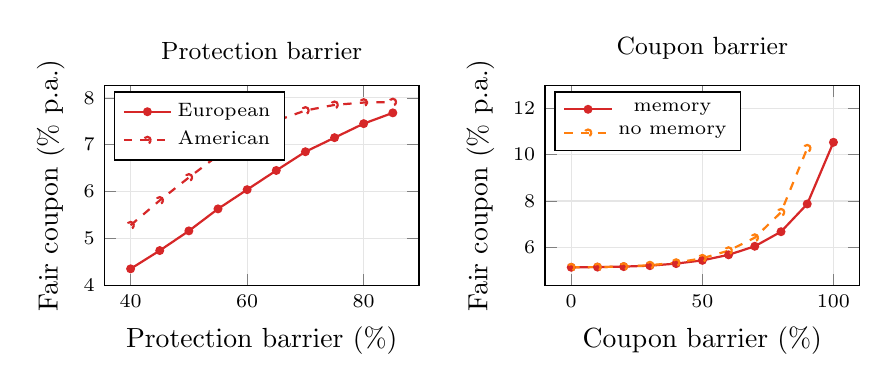
\begin{tikzpicture}
\begin{groupplot}[group style={group size=2 by 1, horizontal sep=1.6cm},
  width=0.46\textwidth, height=0.34\textwidth, ylabel={Fair coupon (\% p.a.)}, grid=major, grid style={gray!20},
  title style={font=\small}, legend style={font=\scriptsize, at={(0.03,0.97)}, anchor=north west}, ticklabel style={font=\scriptsize}]
\nextgroupplot[xlabel={Protection barrier (\%)}, title={Protection barrier}]
\addplot[phoenix, thick, mark=*, mark size=1.2pt] coordinates {(40,4.35) (45,4.74) (50,5.16) (55,5.63) (60,6.04) (65,6.45) (70,6.85) (75,7.15) (80,7.45) (85,7.68)};
\addplot[phoenix, thick, dashed, mark=o, mark size=1.2pt] coordinates {(40,5.28) (45,5.81) (50,6.30) (55,6.77) (60,7.18) (65,7.51) (70,7.73) (75,7.85) (80,7.90) (85,7.91)};
\legend{European, American}
\nextgroupplot[xlabel={Coupon barrier (\%)}, title={Coupon barrier}, ymax=13]
\addplot[phoenix, thick, mark=*, mark size=1.2pt] coordinates {(0,5.13) (10,5.14) (20,5.16) (30,5.20) (40,5.29) (50,5.43) (60,5.67) (70,6.04) (80,6.67) (90,7.87) (100,10.54)};
\addplot[nomemory, thick, dashed, mark=o, mark size=1.2pt] coordinates {(0,5.13) (10,5.14) (20,5.16) (30,5.22) (40,5.33) (50,5.52) (60,5.85) (70,6.41) (80,7.51) (90,10.28)};
\legend{memory, no memory}
\end{groupplot}
\end{tikzpicture}
\caption{Phoenix: fair coupon as a function of the barriers (other features of the base case unchanged; American:
continuous monitoring). Without memory, the fair coupon reaches 23.94\% at a coupon barrier of 100\% (off scale).}
\label{fig:fair_coupon}
\end{figure}

\subsection{Greeks}
Table~\ref{tab:phoenix_greeks} gives the Greeks of five Phoenix variants.

\begin{table}[h]
\centering
\resizebox{\textwidth}{!}{%
\begin{tabular}{@{}lrrrrrrrr@{}}
\toprule
\textbf{Phoenix} & \textbf{Price} & \textbf{Delta} & \textbf{Delta 1\%} & \textbf{Vega} & \textbf{Vanna} & \textbf{Rho} & \textbf{Dividend} & \textbf{Theta} \\
 & & (per point) & (per 1\% move) & (per vol pt) & ($\times 10^{4}$) & (per 1\%) & (per 1\%) & (per day) \\
\midrule
Base & 99.96 & 0.00059 & 0.047 & $-0.335$ & 6.13 & $-0.599$ & $-0.325$ & 0.0050 \\
No memory & 99.67 & 0.00106 & 0.085 & $-0.365$ & 6.27 & $-0.560$ & $-0.357$ & 0.0053 \\
American protection & 99.00 & 0.00229 & 0.184 & $-0.394$ & 5.72 & $-0.448$ & $-0.437$ & 0.0039 \\
Airbag & 101.28 & $-0.00151$ & $-0.121$ & $-0.224$ & 5.38 & $-0.875$ & $-0.101$ & 0.0026 \\
Unconditional coupon & 100.87 & $-0.00077$ & $-0.062$ & $-0.253$ & 5.67 & $-0.745$ & $-0.202$ & 0.0048 \\
\bottomrule
\end{tabular}}
\caption{Greeks of Phoenix variants (nominal 100, coupon 6\%). Base case standard errors: Delta 0.00017, Vega 0.012,
Vanna $0.8 \times 10^{-4}$, Rho 0.044, Dividend 0.044, Theta 0.0014; Gamma and Volga are not significant.}
\label{tab:phoenix_greeks}
\end{table}

The Phoenix is almost Delta-neutral at the money (0.047 for a 1\% move against 0.41 for the Athena): a rise of the
index makes the coupons more likely but also calls the note earlier, which stops a coupon stream priced above par.
When the coupon is well above its fair level, the second effect dominates and the Delta becomes negative (airbag
and unconditional coupon, whose prices are 101.3 and 100.9). The Phoenix is short volatility ($-0.33$ per vol
point) and short dividends ($-0.32$ per point, a third of the Athena): its coupons are paid on a shorter horizon,
so the forward matters less. Figures~\ref{fig:phoenix_greeks} and~\ref{fig:phoenix_profiles} display the Greeks.

\begin{figure}[h]
\centering
\figfile{phoenix_greeks.png}{\textwidth}
\caption{Greeks of the Phoenix variants with 95\% confidence intervals.}
\label{fig:phoenix_greeks}
\end{figure}

\begin{figure}[h]
\centering
\figfile{phoenix_profiles.png}{\textwidth}
\caption{Phoenix: price and Greeks as functions of the spot (30{,}000 paths, spot step 400).}
\label{fig:phoenix_profiles}
\end{figure}

\paragraph{Sensitivities to the Heston parameters.} The base Phoenix has $\partial V/\partial v_0 = -40.4$,
$\partial V/\partial \theta = -44.9$, $\partial V/\partial \kappa = -0.19$, $\partial V/\partial \xi = 1.36$ and
$\partial V/\partial \rho = 0.87$: 58\% to 65\% of the Athena exposures to the variance level.

% ==================================================================
\section{Phoenix versus Athena}\label{sec:comparison}
% ==================================================================
\begin{table}[h]
\centering
\begin{tabular}{@{}lrr@{}}
\toprule
 & \textbf{Athena} & \textbf{Phoenix} \\
 & (annual, snowball) & (quarterly, memory, CB 70\%) \\
\midrule
Fair coupon (\% p.a.) & 9.41 & 6.04 \\
Probability of a call at the first date (\%) & 55.69 & 55.43 \\
Expected life (years) & 2.06 & 1.03 \\
Probability of a capital loss (\%) & 9.06 & 5.22 \\
Expected loss (\% of nominal) & 5.27 & 3.05 \\
Delta (per 1\% move) & 0.407 & 0.047 \\
Vega (per vol point) & $-0.549$ & $-0.335$ \\
Dividend (per 1\% of carry) & $-1.115$ & $-0.325$ \\
\bottomrule
\end{tabular}
\caption{Base cases compared (European protection at 60\%, autocall at 100\%, 4 years); Athena figures from the
companion report \cite{benguedda2026athena}.}
\label{tab:comparison}
\end{table}

The Athena concentrates its coupons in the scenarios where the index is up, which is why its fair coupon is higher
and its Delta almost nine times larger; the Phoenix pays regularly as long as the index stays above 70\%, a more stable
income for a lower rate. With the same quarterly dates, the snowball Athena and the memory Phoenix with
$B^{\mathrm{cpn}} = B^{\mathrm{call}}$ have the same fair coupon (10.54\%), which is the identity of
Section~\ref{sec:products}.

% ==================================================================
\section{Implementation}\label{sec:implementation}
% ==================================================================

\subsection{Code}
\begin{itemize}
\item \code{Products/Phoenix/phoenix.py}: the self-contained class \code{Phoenix} (contract, \code{path\_payoff},
\code{fair\_coupon}, \code{statistics});
\item \code{Equity\_Models/monte\_carlo.py}: \code{MonteCarloPricer}, which simulates the paths and calls
\code{path\_payoff} for products with several cash flows;
\item \code{Equity\_Models/Heston.py}, \code{Equity\_Models/forward\_curve.py}: calibrated model and forward curve;
\item \code{Equity\_Models/greeks.py}: Greeks with common random numbers, including the Dividend Greek;
\item \code{Products/market.py}: CAC40 market data and calibrated Heston model (\code{cac40\_heston});
\item \code{Products/notes\_analysis.py}: comparison of variants and plots;
\item notebook \code{Products/Phoenix/phoenix\_pricer.ipynb}.
\end{itemize}

\begin{lstlisting}
from market import cac40_heston
from phoenix import Phoenix
from Equity_Models.monte_carlo import MonteCarloPricer
from Equity_Models.greeks import Greeks

mkt = cac40_heston()
pricer = MonteCarloPricer(n_paths=50_000, steps_per_year=52, seed=42)
note = Phoenix(4.0, mkt.S0, 0.06, coupon_barrier=0.7, memory=True, frequency=0.25,
               autocall_barrier=1.0, protection_barrier=0.6, protection_type="european")
print(pricer.price(mkt.heston, note))              # price and standard error
print(note.fair_coupon(pricer, mkt.heston))        # coupon p.a. at par
print(note.statistics(pricer, mkt.heston))         # call probabilities, loss, life, coupons
print(Greeks(pricer).compute(mkt.heston, note, Greeks.ORDER))
\end{lstlisting}

\subsection{Cost}
With $N$ paths and $M$ steps, the simulation costs $\mathcal{O}(NM)$ in time and stores $S$ and $v$, i.e.
$16(M+1)N$ bytes: 167 MB for $N = 50{,}000$ and the weekly grid of 4 years, 807 MB on a daily grid. Following the
note through its $n$ observation dates costs $\mathcal{O}(nN)$, the American continuous protection
$\mathcal{O}(NM)$. Measured times (one CPU core): 0.30 s for a valuation including the simulation; 0.02 to 0.12 s
for the price, the fair coupon and the statistics of a variant on cached paths (1.5 s with an American
protection); 26 s for the eight Greeks of five notes (14 valuations each); 41 to 44 s for the spot profiles of
four notes (16 spots $\times$ 6 scenarios, 30{,}000 paths).

% ==================================================================
\section{Limitations and Next Steps}\label{sec:limitations}
% ==================================================================
\begin{itemize}
\item \emph{Single underlying.} Most autocalls sold today are worst-of on two to four indices or stocks; they need
a multi-asset model and a correlation calibration.
\item \emph{Model.} The value of an autocall depends on the forward skew and on the joint dynamics of spot and
volatility between observation dates; a pure Heston model with constant parameters is not the market standard,
which is a local stochastic volatility model calibrated to the whole surface \cite{bergomi2016}.
\item \emph{Fair coupon.} It prices the note at par without issuer margin, funding spread or issuer credit risk; a
real issue price is below par by the margin.
\item \emph{Discretisation.} Euler full truncation with the Feller condition violated ($2\kappa\theta/\xi^2 = 0.49$),
weekly grid with the variance frozen over each week for the Brownian bridge.
\item \emph{Greeks.} Gamma and Volga are not significant with 50{,}000 paths: the payoff jumps at the coupon,
autocall and protection barriers.
\item \emph{Dividends.} Continuous dividend yield bootstrapped from the forwards; real notes are exposed to
discrete dividends and to dividend risk, which the Dividend Greek only measures for a parallel shift.
\end{itemize}

% ==================================================================
\section{Conclusion}
% ==================================================================
A single parametrisation covers the Phoenix with all its usual features, and a Monte Carlo pricer under a calibrated
Heston model recovers two exact limit cases within one standard error and the exact identity with the snowball
Athena. On the CAC40 of 12 February 2025, the base 4-year Phoenix pays 6.04\% a year; its zero-coupon part is the
same as the Athena one, and its lower coupon only reflects that a unit coupon is worth 1.75 times more. The coupon
barrier and the protection are the main drivers of the fair coupon, the memory is worth 0.37 point at a barrier of
70\%, and everything that shortens the life of the note (more frequent observations, step-down) raises the fair
coupon. The note is almost Delta-neutral at the money, short volatility and short dividends, a third of the Athena on
dividends.

% ==================================================================
\appendix
\section{Notation}
% ==================================================================
\begin{center}
\begin{tabular}{@{}ll@{}}
\toprule
Symbol & Meaning \\
\midrule
$N$, $\Sref$, $T$ & Nominal, initial fixing, maturity \\
$t_k$, $\delta_k = t_k - t_{k-1}$ & Observation dates and accrual periods \\
$P_k = S_{t_k}/\Sref$ & Performance at $t_k$ \\
$B^{\mathrm{call}}_k$, $B^{\mathrm{cpn}}_k$, $B^{\mathrm{prot}}$ & Autocall, coupon and protection barriers (fractions of $\Sref$) \\
$m_i$ & Number of coupon periods paid at $t_i$ (memory) \\
$c$, $c^\star$ & Coupon rate per annum, fair coupon \\
$K_{\mathrm{put}}$, $\phi$ & Strike of the short put, capital floor \\
$\tau$ & Call date \\
$\ind_{\mathrm{KI}}$ & Knock-in event of the protection \\
\bottomrule
\end{tabular}
\end{center}

% ==================================================================
\begin{thebibliography}{99}
\bibitem{benguedda2026athena} E. Benguedda, \emph{Athena Autocallable Notes on the CAC40 under a Calibrated Heston
Model: Fair Coupons, Scenarios and Greeks}, 2026.
\bibitem{benguedda2026heston} E. Benguedda, \emph{Calibration of the Heston Stochastic Volatility Model: Theoretical
Framework, Numerical Methods, and Limitations}, 2026.
\bibitem{benguedda2026barrier} E. Benguedda, \emph{Monte Carlo Pricing and Greeks of Single Barrier Options under a
Calibrated Heston Model}, 2026.
\bibitem{heston1993} S. L. Heston, A closed-form solution for options with stochastic volatility with applications
to bond and currency options, \emph{Review of Financial Studies}, 6(2):327--343, 1993.
\bibitem{bouzoubaa2010} M. Bouzoubaa and A. Osseiran, \emph{Exotic Options and Hybrids: A Guide to Structuring,
Pricing and Trading}, Wiley, 2010.
\bibitem{bergomi2016} L. Bergomi, \emph{Stochastic Volatility Modeling}, Chapman and Hall/CRC, 2016.
\bibitem{glasserman2004} P. Glasserman, \emph{Monte Carlo Methods in Financial Engineering}, Springer, 2004.
\bibitem{beaglehole1997} D. R. Beaglehole, P. H. Dybvig and G. Zhou, Going to extremes: correcting simulation bias
in exotic option valuation, \emph{Financial Analysts Journal}, 53(1):62--68, 1997.
\bibitem{reiner1991} E. Reiner and M. Rubinstein, Breaking down the barriers, \emph{Risk}, 4(8):28--35, 1991.
\bibitem{andersen2008} L. Andersen, Simple and efficient simulation of the Heston stochastic volatility model,
\emph{Journal of Computational Finance}, 11(3):1--42, 2008.
\end{thebibliography}

\end{document}
